\documentclass{article}

\usepackage[english]{babel}
\usepackage[utf8]{inputenc}
\usepackage{amsmath}
\usepackage{amsthm}
\usepackage{amssymb}
\usepackage{mathtools}
\usepackage{amsfonts}
\usepackage{subcaption}
\usepackage{graphicx}
\usepackage{wrapfig}
\usepackage{bbm}
\usepackage{dsfont}
\usepackage{listings}

% set up margin
\usepackage
[
  a4paper,
  left=3cm,
  right=3cm,
  top=3cm,
  bottom=3cm,
]
{geometry}

% set up header
\usepackage{fancyhdr}
\pagestyle{fancy}
\fancyhf{}
\lhead{6.438 Algorithms for Inference}
\chead{Problem Set 4}
\rhead{Hongzi Mao}
\cfoot{\thepage}
\rfoot{\footnotesize{\emph{Collaborated with: Hongzhou Ye, Zhiwei Ding}}}

% footer line
\renewcommand{\footrulewidth}{0.4pt}

% sans serif italic
\newcommand{\s}[1]{\textsf{\textit{#1}}}

% bold face sans serif
\newcommand{\bs}[1]{\textsf{\textbf{#1}}}

% set symbol
\usepackage[mathscr]{euscript}

% empty set
\let\emptyset\varnothing

% qed
\newcommand{\qeds}{\hfill\qedsymbol}

% math bold face
\newcommand{\bm}{\mathbf}

% argmax
\DeclareMathOperator*{\argmax}{argmax}

% independence symbol
\makeatletter
\newcommand*{\indep}{%
  \mathbin{%
    \mathpalette{\@indep}{}%
  }%
}
\newcommand*{\nindep}{%
  \mathbin{%                   % The final symbol is a binary math operator
    \mathpalette{\@indep}{\not}% \mathpalette helps for the adaptation
                               % of the symbol to the different math styles.
  }%
}
\newcommand*{\@indep}[2]{%
  \sbox0{$#1\perp\m@th$}%        box 0 contains \perp symbol
  \sbox2{$#1=$}%                 box 2 for the height of =
  \sbox4{$#1\vcenter{}$}%        box 4 for the height of the math axis
  \rlap{\copy0}%                 first \perp
  \dimen@=\dimexpr\ht2-\ht4-.2pt\relax
  \kern\dimen@
  {#2}
  \kern\dimen@
  \copy0 %                       second \perp
} 
\makeatother

%%%%%%%%%%%%%%%%%%%%%%%%%%%%%%%%%%%%%%%%%%%%%%%%%%%%%%%%%%%%%%%%%%%%%%%%
%%%%%%%%%%%%%%%%%%%%%%%%% Begin document here %%%%%%%%%%%%%%%%%%%%%%%%%%
%%%%%%%%%%%%%%%%%%%%%%%%%%%%%%%%%%%%%%%%%%%%%%%%%%%%%%%%%%%%%%%%%%%%%%%%
\begin{document}
 
\section*{Problem 4.5}
%
(a) At each loopy BP step, the message follows
\begin{align*}
	m_{j\to i}(x_i) = \sum_{x_j}\exp(\beta x_i x_j)\prod_{k\in \partial j \backslash i} m_{k\to j}(x_j),
\end{align*}
where $\partial j$ denotes the four neighboring nodes of $j$.
\\

\noindent
(b) Assume the message is invariant under translation, we have
\begin{align*}
	m(1) &= \exp(\beta)m(1)^3 + \exp(-\beta)m(-1)^3\\
	m(-1) &= \exp(-\beta)m(1)^3 + \exp(\beta)m(-1)^3.
\end{align*}
%

Therefore, 
\begin{align}
	m(x) = \exp(\beta)m(x)^3 + \exp(-\beta)m(-x)^3. \label{eq:5b}
\end{align}
\\

\noindent
(c) Massaging terms in $h$, we have
\begin{align*}
	m(1) &= \exp(2\beta h)m(-1)\\
	m(-1) &= \exp(-2\beta h)m(1).
\end{align*}
%

Since $Z = m(1) + m(-1)$,
\begin{align*}
	Z &= m(1) + \exp(-2\beta h)m(1)\\
	Z &= \exp(2\beta h)m(-1) + m(-1).
\end{align*}
%

Thus,
\begin{align}
	m(x) = \frac{Z}{1 + \exp(-2\beta h x)}. \label{eq:5c}
\end{align}
%

Now we plug in results from (b) for $m(1) / m(-1)$, we have
\begin{align*}
	\exp(2\beta h) = \frac{m(1)}{m(-1)} &=
	\frac{\exp(\beta)m(1)^3 + \exp(-\beta)m(-1)^3}{\exp(-\beta)m(1)^3 + \exp(\beta)m(-1)^3} \\
	&=\frac{\frac{\exp(\beta)Z^3}{\big[1 + \exp(-2\beta h)\big]^3} +
	  \frac{\exp(-\beta)Z^3}{\big[1 + \exp(2\beta h)\big]^3}}
	  {\frac{\exp(-\beta)Z^3}{\big[1 + \exp(-2\beta h)\big]^3} + 
	  \frac{\exp(\beta)Z^3}{\big[1 + \exp(2\beta h)\big]^3}}\\
	&=\frac{\frac{\exp(\beta)\exp(6\beta h)}{\big[\exp(2\beta h) + 1\big]^3} +
	  \frac{\exp(-\beta)}{\big[1 + \exp(2\beta h)\big]^3}}
	  {\frac{\exp(-\beta)\exp(6\beta h)}{\big[\exp(2\beta h) + 1\big]^3} + 
	  \frac{\exp(\beta)}{\big[1 + \exp(2\beta h)\big]^3}}\\
	&=\frac{\exp(\beta)\exp(3\beta h) +
	        \exp(-\beta)\exp(-3\beta h)}
	       {\exp(-\beta)\exp(3\beta h) +
	        \exp(\beta)\exp(-3\beta h)}.
\end{align*}
%

Finally,
\begin{align*}
	\tanh(\beta h) &= \frac{\exp(2\beta h) - 1}{ \exp(2\beta h) + 1} \\
	&= \frac{\frac{\exp(\beta)\exp(3\beta h) +
	        \exp(-\beta)\exp(-3\beta h)}
	       {\exp(-\beta)\exp(3\beta h) +
	        \exp(\beta)\exp(-3\beta h)} - 1}
	        {\frac{\exp(\beta)\exp(3\beta h) +
	        \exp(-\beta)\exp(-3\beta h)}
	       {\exp(-\beta)\exp(3\beta h) +
	        \exp(\beta)\exp(-3\beta h)} + 1} \\
    &= \frac{\exp(\beta)\exp(3\beta h) + \exp(-\beta)\exp(-3\beta h) -
             {\exp(-\beta)\exp(3\beta h) - \exp(\beta)\exp(-3\beta h)}}
            {\exp(\beta)\exp(3\beta h) + \exp(-\beta)\exp(-3\beta h) +
             {\exp(-\beta)\exp(3\beta h) + \exp(\beta)\exp(-3\beta h)}} \\
    &= \frac{\big[\exp(\beta) - \exp(-\beta)\big]
             \big[\exp(3\beta h) - \exp(-3\beta h)\big]}
            {\big[\exp(\beta) + \exp(-\beta)\big]
             \big[\exp(3\beta h) + \exp(-3\beta h)\big]}\\
    &= \tanh(\beta) \tanh(3\beta h).
\end{align*}\qeds
\\

\noindent
(d) Since $m(x) = Z/\big(1 + \exp(-2\beta h x)\big)$, we only need to determine the value
of $\beta h$ to find the fixed message. We denote $k = \beta h$. Notice from (c) that
\begin{align*}
	\frac{\tanh(k)}{\tanh(3k)} = \frac{\tanh(\beta h)}{\tanh(3\beta h)} = \tanh(\beta).
\end{align*}
%
\begin{figure}[h]
  \centering
  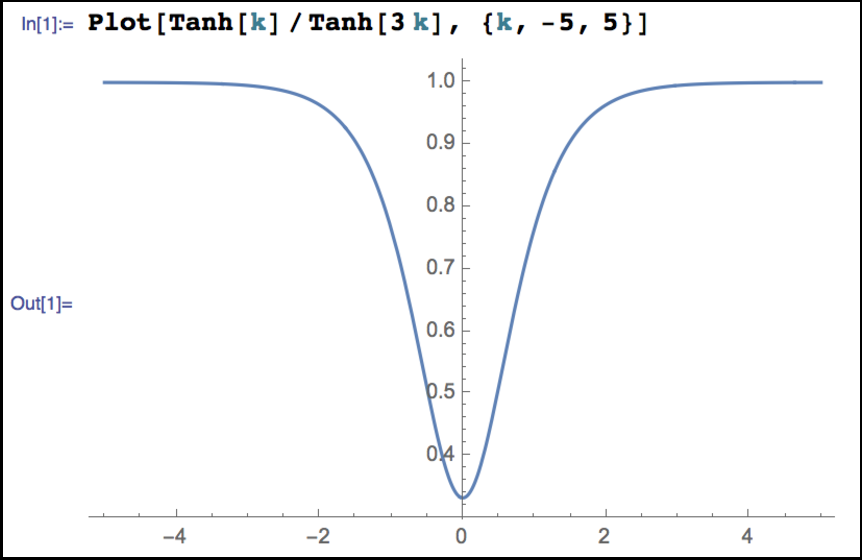
\includegraphics[width=0.4\columnwidth]{5d.pdf}
    \vspace{-0.1cm}
  \caption{$\tanh(k)/\tanh(3k)$, plotted over $k\in(-5,5)$. The intersection with y-axis is at $1/3$.}
  \label{f:5d}
\end{figure}
%

To find the solution fo $k$ is equivalent to find the intersection of $\tanh(k)/\tanh(3)$ and $\tanh(\beta)$.
We first note that $\tanh(0) = 0$, and $\tanh'(k) = \text{sech}(k)$ and $\tanh'(3k) = 3\text{sech}(k)$,
applying L'Hospital's Rule,
\begin{align*}
	\lim_{k\to 0} \frac{\tanh(k)}{\tanh(3k)} = \lim_{k\to 0} \frac{\tanh'(k)}{\tanh'(3k)} = \lim_{k\to 0} \frac{\text{sech}(k)}{3\text{sech}(k)} = \frac{1}{3}.
\end{align*}

Second, note that $\tanh(k)/\tanh(3k)$ is symmetric, i.e., 
\begin{align*}
	\frac{\tanh(-k)}{\tanh(-3k)} = \frac{-\tanh(k)}{-\tanh(3k)} = \frac{\tanh(k)}{\tanh(3k)}.
\end{align*}

Lastly, $\tanh(k)/\tanh(3k)$ increases monotonically for $k>0$ (and decreases monotonically for $k<0$).
This is  because we can write
\begin{align*}
	\frac{\tanh(k)}{\tanh(3k)} &= \frac{\exp(k) - \exp(-k)}{\exp(k) + \exp(-k)}
	\times\frac{\exp(3k) + \exp(-3k)}{\exp(3k) - \exp(-3k)}\\
	&=\frac{\exp(k) - \exp(-k)}{\exp(k) + \exp(-k)}\times
	\frac{\exp(k) + \exp(-5k)}{\exp(k) - \exp(-5k)}.
\end{align*}
Here, as $k>0$ increases, $\exp(-k)$ gets increasingly smaller; and $\exp(-k)$ always overwhelms $\exp(-5k)$.
As a result, $\tanh(k)/\tanh(3k)$ monotonically increases for $k>0$. The upper bound for this expression is
\begin{align*}
	\lim_{k\to\infty}\frac{\tanh(k)}{\tanh(3k)} &= 
	\lim_{k\to\infty}\frac{\exp(k) - \exp(-k)}{\exp(k) + \exp(-k)}
	\times\lim_{k\to\infty}\frac{\exp(3k) + \exp(-3k)}{\exp(3k) - \exp(-3k)}\\
	&= \lim_{k\to\infty}\frac{1 - \exp(-2k)}{1 + \exp(-2k)}
	\times\lim_{k\to\infty}\frac{1 + \exp(-6k)}{1 - \exp(-6k)}\\
	&= 1.
\end{align*}

Figure~\ref{f:5d} visualizes $\tanh(k)/\tanh(3k)$. Therefore, when $\tanh(\beta) > 1/3$ (notice 
$\lim_{\beta\to\pm\infty}\tanh(\beta)=1$), $\tanh(k)/\tanh(3k) = \tanh(\beta)$ will have two
symmetric solutions. Moreover, since $m(x) = 0$ is always a solution (not expressed by Equation~\eqref{eq:5c}),
the LBP has three distinct fixed points. \qeds
\\

\noindent
(e)
\end{document}